\documentclass[a4paper,twoside]{articlewithlogo}
\usepackage{pdfpages}
\usepackage[titletoc,toc,page]{appendix}
\usepackage{enumerate}
\usepackage{graphicx}
\graphicspath{{Figuras/}}
\usepackage{color}
\usepackage[cmex10]{amsmath}
\usepackage{array}
\usepackage{float}
\usepackage[utf8]{inputenc} 
\usepackage[portuguese]{babel}
\usepackage[font=normalsize,format=plain,labelfont=bf,up,textfont=up,figurename=Figura,tablename=Tabela]{caption}
\usepackage{subcaption}
\usepackage[top=1in, bottom=1in, left=1.25in, right=1.25in]{geometry}
\usepackage{indentfirst}
\usepackage{fancyhdr}
% Font packages
\usepackage{amssymb}
\usepackage{amsfonts}
\usepackage{steinmetz}
% Nice extra font package, e.g. \mathds{1}
\usepackage{dsfont}
\usepackage{color}
\usepackage{blindtext}
% Use multiple rows when writing tables
\usepackage{multirow}
\usepackage{booktabs}
\usepackage{bigstrut}
% Uncomment next line to make footnots per page
\usepackage{perpage}
% Uncoment next group of lines to create the table of contents for the PDF
\usepackage{hyperref}
\definecolor{darkblue}{rgb}{0,0,0.5}
\renewcommand{\title}{Trabalho de Automação Industrial}
\newcommand{\subtitle}{Seleção de Peças 2}
\hypersetup{
    pdftitle={\title},
    pdfauthor={},
    bookmarksnumbered=true,     
    bookmarksopen=true,         
    bookmarksopenlevel=1,       
    colorlinks=true,
    linkcolor=darkblue,
    filecolor=darkblue,  
    urlcolor=darkblue,  
    citecolor=darkblue,              
    pdfstartview=Fit,          
    pdfpagemode=UseOutlines,    % this is the option you were lookin for
    pdfpagelayout=TwoPageRight
}
\let\oldcontentsline\contentsline%
\renewcommand\contentsline[4]{%
    \oldcontentsline{#1}{\smash{\raisebox{1em}{\hypertarget{toc#4}{}}}#2}{#3}{#4}}

\newcommand\mysection[1]{\section[#1]{\protect\hyperlink{tocsection.\thesection}{#1}}}
\newcommand\mysubsection[1]{\subsection[#1]{\protect\hyperlink{tocsection.\thesection}{#1}}}

\newcommand{\conteudo}{\tableofcontents\label{tocsection}}


\pagestyle{fancy}


\fancyhead[CO]{\title}
\fancyhead[CE]{\subtitle}
\fancyhead[R]{}
\fancyhead[L]{}
\fancyfoot[C]{\thepage}

\allowdisplaybreaks

\newif\ifdebug
\newcommand\todo[1]{\ifdebug {\color{red}#1}\fi}
\renewcommand{\appendixtocname}{Ap\'endices}
\renewcommand{\appendixpagename}{Ap\'endices}
\debugfalse
\begin{document}
\large
\todo{REMEMBER TO TURN DEBUG OFF}
\begin{titlepage}
\begin{center}
% Upper part of the page. The '~' is needed because \\
% only works if a paragraph has started.

\includegraphics[width=40mm]{logos/minerva2.png}%~\\[0.5cm]
\vspace{50pt}
% Title
\rule{\linewidth}{0.5mm} \\[0.4cm]
{ \huge \bfseries \title \\[0.4cm] }
\rule{\linewidth}{0.5mm} \\[0.5cm]
\textsc{\Large \subtitle}\\[1.5cm]
\vspace{60pt}
% Author and supervisor
\begin{minipage}{0.4\textwidth}
\center
 \large
\textbf{Felipe Matheus \\Philipe Miranda\\Rafael Accácio }\\
%NOME DOS ALUNOS
\end{minipage}
\vfill
% Bottom of the page
{\large \today}
\end{center}
\end{titlepage}
\conteudo
\newpage
\mysection{Motivação}
Com o constante avanço das indústrias e a automatização dos processos, é de suma importância o conhecimento de como funcionam controle de eventos discretos, muito utilizado em diversas áreas, dos setores agrícolas e alimentos até aos automotivos e aeronáuticos. Com isso, foi realizado um trabalho com o fim de realizar tal tipo de controle em uma planta de pequena escala, com fim de preparar os alunos para o trabalho cotidiano na área de automação industrial.
\mysection{Introdução e Objetivo}
Este relatório tem como objetivo mostrar o trabalho realizado para a matéria Automação Industrial do controle de uma planta mecatrônica educacional do fabricante Christiani-Technical Institute for Vocational Training. 
A seção da planta que foi trabalhada é a de seleção dos blocos. E a ordem dos blocos a serem selecionados são 2 de metal com a concavidade voltada para cima e 1 de plástico com a concavidade para baixo.
As especificações do trabalho podem ser vistas a seguir:
\paragraph{$2^o$ Trabalho - Sistema de seleção de peças II.\\}
Considere um sistema de seleção de peças com dois alimentadores. O alimentador 1
fornece apenas peças plásticas e o alimentador 2 apenas peças metálicas. Deve ser sempre
fornecido duas peças metálicas em sequência e depois uma plástica. Caso seja entregue
a sequência errada, a peça deve ser rejeitada, ou seja, deve chegar até o fim da esteira e
depois retornar até sair da esteira. A peça plástica deve estar com o encaixe voltado para
baixo e a peça metálica com o encaixe voltado para cima. Considere ainda a existência de
três botões: QUIT, STOP e START. O sistema é iniciado ao pressionar o botão START.
Caso o botão STOP seja pressionado o sistema para como está e depois reinicia de onde
parou com um novo pressionar do START. Caso o botão QUIT seja pressionado, o sistema
retorna ao estado inicial.
\\
Para fazer o trabalho, primeiramente construímos uma rede de petri, depois transformamos em um Grafcet e finalmente transformamos a rede de petri em um programa Ladder a partir de algoritmo de conversão apresentado pelo professor Marcos e depois o programa foi gravado em um Controlador Lógico Programável e testado.
\newpage
\eject \pdfpagewidth=28in \pdfpageheight=12in
\mysection{Rede de Petri}
\begin{figure}[H]
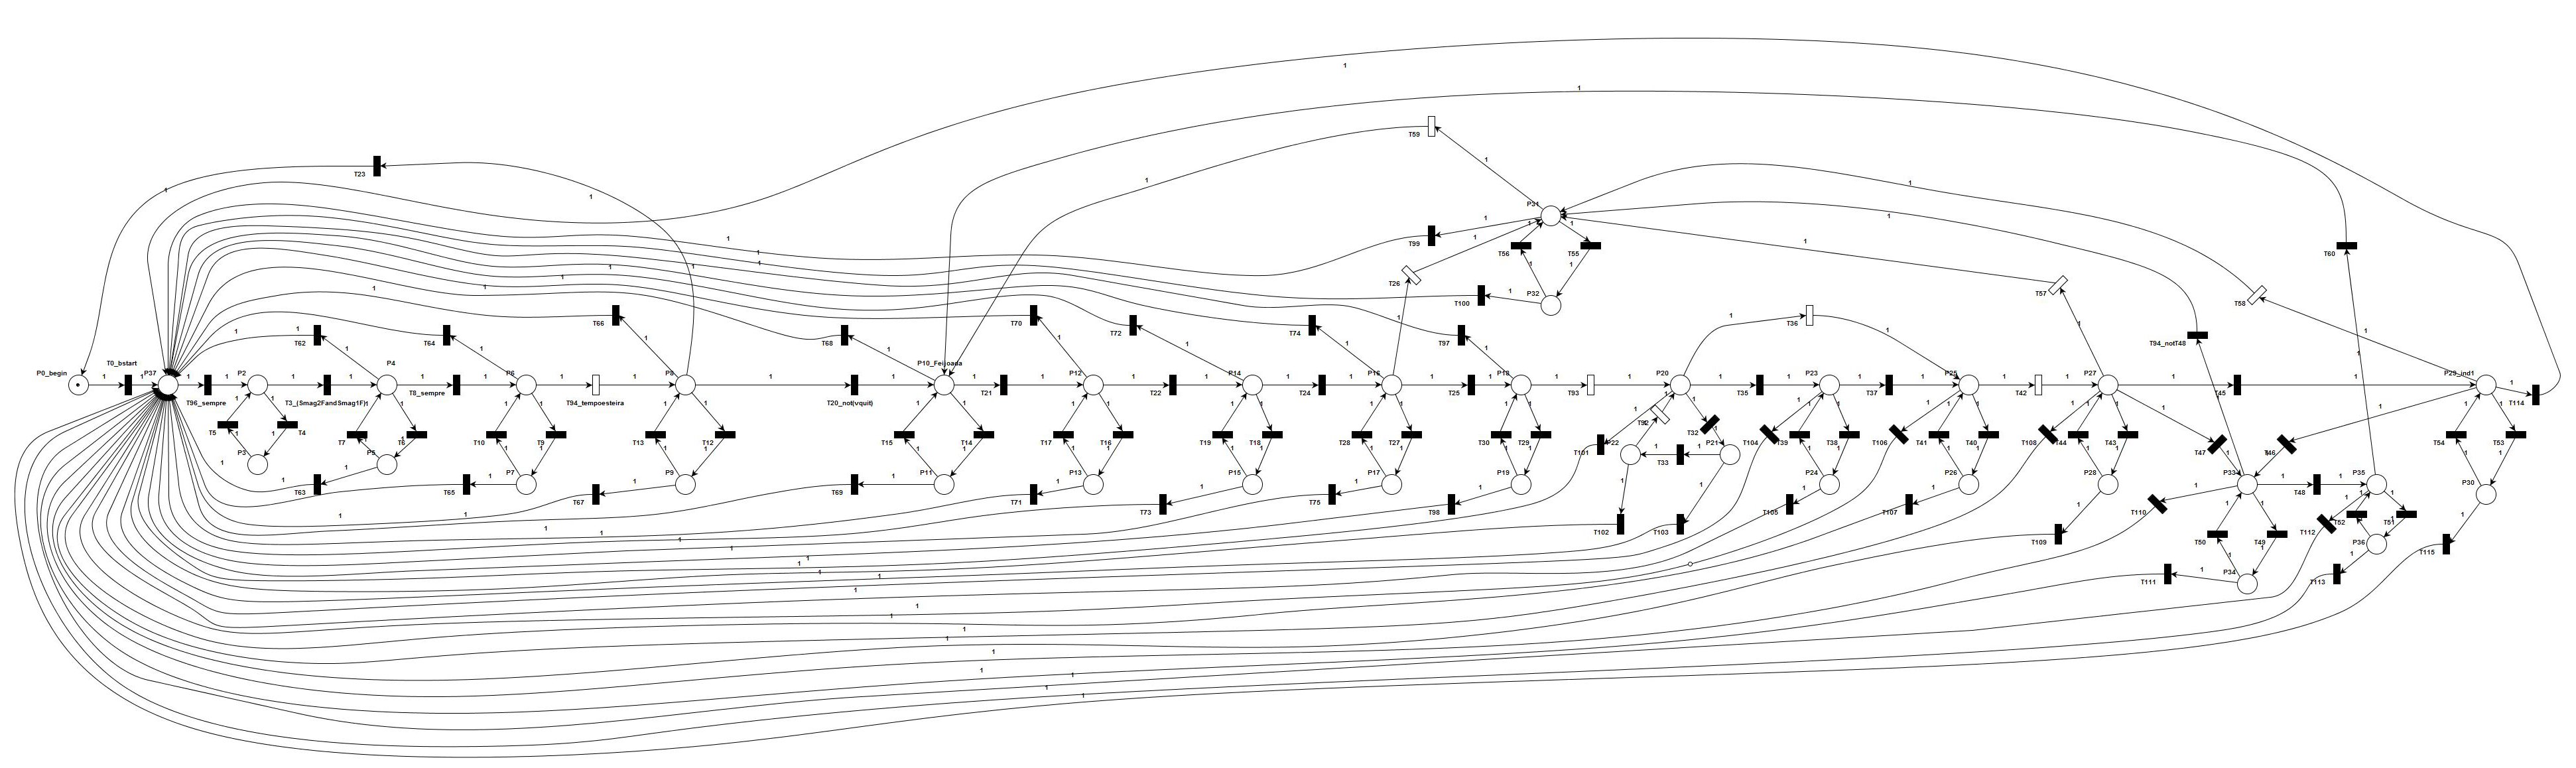
\includegraphics[width=25in]{petri.png}
\caption{Rede de Petri}
\label{rededepetri}
\end{figure}
\eject \pdfpagewidth=210mm \pdfpageheight=297mm
\newpage
Podemos ver na figura \ref{rededepetri} a rede petri que foi construída para seguir o que foi especificado no problema. A seguir iremos explicar os estados e as etapas de cada parte da rede.

\subsection{Decisões de projeto} Antes das devidas explicações de cada estado, há de se citar cinco preocupações importantes no projeto que foram fundamentais para caracterizar tal rede de petri. 

\subsection*{Transições} Na rede de Petri apresentada, as transições brancas representam transições que envolvem temporizadores, usadas para timeouts -- como no caso do estado de "roubo", que será explicado adiante -- e para dar tempo de os objetos envolvidos na ação se movimentarem -- como no caso do pistão verificador de concavidade. Já as transições pretas são as que acontecem pelo sinal de um ou mais sensores ou variáveis.

\subsection*{Variável \textit{Blocos}} A segunda decisão, e fundamentalmente ligada ao objetivo do problema, foi a criação de uma variável chamada \textit{blocos}, cuja função é a de contar quantos blocos de plástico e metal já passaram e qual seria a próxima transição a ser tomada dependendo do valor da mesma. Essa decisão foi tomada para atender o pedido da questão de 2 peças de metal com o encaixe para cima e dois para baixo. Conseguimos garantir isso através da seguinte lógica booleana.

\begin{equation}
	((blocos<2).ind.cima)+((blocos==2).ind'.cima')
	\label{eq:logicadeblocos}
\end{equation}

Onde a variável \textit{ind} indica se é metal caso seja 1 e plástico caso 0, enquanto a variável \textit{cima} indica que a peça está virada para cima caso 1, e para baixo caso 0. Assim caso a expressão acima seja verdadeira, ocorrerá uma transição que levará a um estado (dependendo do valor de \textit{ind}) onde a variável blocos será incrementada monotonicamente, e o processo recomeçará (caso a variável passe o valor de 2, seu valor será resetado para 0 e o processo recomeçará).

\subsection*{Estado de ``roubo'' (P31)} Outra preocupação foi baseada na possibilidade de ocorrer um possível ``roubo" ou ``sumiço" de peça, para isso em estados onde poderia acontecer tal fato foi inserida uma transição temporal a um estado onde o sistema age a fim de consertar o problema do desaparecimento da peça. Esse estado se caracteriza por assegurar que o atuador do sensor de profundidade seja levantado, e que a esteira percorra o caminho inverso durante 12s (tempo suficiente para percorrer o percurso inteiro de volta). E após um tempo levemente maior que 12 segundos, a transição T59 será ativada garantindo que a ficha retorne ao estado que começa o procedimento de envio de peça.

\subsection*{Quits}Em terceiro lugar cogitamos o acionamento do botão ``quit", que exerceria a função de parar o processo onde quer que ele esteja e voltar ao estado P37, responsável por retornar o \textit{default} de todas as variáveis do sistema exceto a variável \textit{blocos}, junto com o acionamento reverso da esteira durante 12 segundos (para rejeitar qualquer peça que esteja na esteira) combinado com a contração dos atuadores por medidas de segurança do equipamento.
\\
Relacionada a decisão do \textit{quit} foi atribuída a variável \textit{vquit}, cujo dafault é 0 e a transição para 1 é feita através do botão \textit{quit} presente na planta. Essa variável assumindo valor positivo sinaliza que o sistema está no processo de saída da operação, e apenas retornará ao funcionamento normal após passar pelo estado P37, que fara \textit{vquit} assumir o valor de 0 novamente.

\subsection*{Stops e Starts}Por fim veio a preocupação caso o botão Stop venha a ser pressionado em todos os possíveis estados. Para isso, todos os estados (com exceção de P0 e P37) possuem um ``estado espelho'' (O estado espelho de P2 é P3, de P4 é P5, e assim sucessivamente seguindo a Figura \ref{rededepetri}), onde as fichas são transmitidas para lá através do \textit{stop} e voltam ao anterior através do \textit{start}. Com exceção apenas do estado P20, que é o estado onde o atuador do sensor de profundidade é estendido, então nesse caso se o botão \textit{stop} é pressionado durante o estado da extensão, ele irá para um estado onde seu \textit{start} levará a um terceiro ``estado espelho" que fará a retração do atuador novamente antes de voltar ao original por uma transição temporal (T92). Vale ressaltar também que todas as demais transições que não envolvam os ``estados espelhos" são um \textit{and} booleano entre um \textit{not(stop)} e a transição respectiva.
\\
Para completar a explicação do \textit{stop}, falaremos sobre a variável criada \textit{vstop}. Ela é caracterizada por assumir o valor de 1 quando o botão \textit{stop} da planta for pressionado e voltar ao valor de 0 quando o botão \textit{start} for pressionado. Esse passo foi importante para a implementação dos ``estados espelhos", pois conseguimos identificar através dessa variável quando o sistema está parado (\textit{vstop} = 1) ou em execução (\textit{vstop} = 0). E caso desejemos voltar de onde paramos, pressionamos o botão de \textit{start}, alterando a variável \textit{vstop}, fazendo a voltar volte a ser 0.


\subsection{Estados característicos} Falaremos agora sobre os estados mais relevantes da rede de petri.

\subsection*{P10}Esse estado é de suma importância para a rede, pois ele é o início do procedimento pedido no enunciado. Ele será alcançado de 3 maneiras, através do acionamento de T20, que caracteriza o fim do procedimento de inicialização; através do acionamento de T60 (cuja condição é a equação \eqref{eq:logicadeblocos}), simbolizando o término de um processo inteiro da esteira e acréscimo na variável \textit{blocos}, devido ao estado P35; e pela T59, uma transição temporária após o estado P31, estado que caracteriza o desaparecimento de uma peça.

\subsection*{P0 begin} Esse é o estado que originalmente possui a ficha do sistema, ele será alcançado apenas se o \textit{quit} não tiver sido acionado antes do sistema terminar sua inicialização. Após o acionamento da transição T0 (pelo botão \textit{start}) a rede começará seu processo de inicialização que consiste na verificação dos valores das variáveis, contração dos atuadores e no retorno de 12s da esteira, por medidas de segurança do sistema.

\subsection*{P31} Estado do desaparecimento da peça. Ele é alcançado através de uma contagem de 3 transições temporárias caracterizadas pela perda ou retirada da peça. E através da T94, que consiste no não acionamento da T48 (explicação no estado P33).
Sua atitude será a de repassar a ficha para P10 através da T59.

\subsection*{P37} Estado da inicialização da rede. Ele receberá a ficha do quit de todos os estados e do estado de desaparecimento. Será responsável por repassar a ficha pelos próximos 4 estados antes de P10, estados esses cuja função é reinicializar as variáveis (exceto \textit{blocos}), contraindo atuadores e revertendo a esteira, garantindo assim a segurança do procedimento.

\subsection{Demais estados} Por fim explicaremos os demais estados.

\subsection*{P16} Estado de inicialização da esteira após receber a peça de metal ou plástico. Os estados entre P10 e P16 possuem a função de colocar a peça na esteira vinda da unidade de armazenamento, através da ativação e contração dos atuadores presentes na mesma.

\subsection*{P20 P21 P22} Estados responsáveis pela detecção da concavidade. P20 é o estado original e P21 junto com P22 são os ``estados espelhos" caso \textit{stop} seja pressionado. P20 irá parar a esteira e acionar o atuador do sensor de profundidade, caso ele encoste na peça, a transição T35 será acionada levando para P23, caso contrário a transição temporal T36 será ativada levando para P25. 

\subsection*{P23 P25} P23 é estado que altera a variável \textit{cima}, essencial para a lógica booleana da equação \eqref{eq:logicadeblocos}. Ele estabelece \textit{cima} = 1 e ativa a transição T37 para seguir ao estado P25, este último responsável por retrair o atuador do sensor de profundidade.

\subsection*{P27} Retornará o movimento da esteira, e dependendo de 3 transições ele poderá mudar para P29, P33 ou P31. 
T57 é uma transição temporal e será acionada enviando a ficha para P31 caso a peça desapareça. No caso, se nenhuma transição for ativada em 10 segundos.
T45 será ativada caso o sensor indutivo detecte a presença metálica, encaminhando a ficha para o estado P29.
T47 será ativada caso o sensor de fim de curso detecte a presença de uma peça, levando a ficha para P33.

\subsection*{P29} Mudará a variável \textit{ind} para 1, indicando que a peça é metálica, isso é necessário para a lógica da equação \eqref{eq:logicadeblocos}. Nesse estado, além dos casos das transições de \textit{quit} e \textit{stop}, poderão ocorrer a transição T46 e T58.
T46 é acionada caso o sensor de fim de curso detecte a presença de uma peça, movendo a ficha para o estado P33, e caso nenhuma transição seja acionada em 10s, ocorrerá T58 enviando a ficha para o estado P31, representando o desaparecimento da peça.

\subsection*{P33} P33 é o estado onde existe uma peça no final da esteira, detectada pelo sensor de fim de curso. Nesse estado ocorrerá a verificação da condição do problema, da sequência de 2 peças metálicas com concavidade para cima e uma metálica com concavidade para baixo. Caso essa condição booleana seja atendida, a transição T48 será acionada, enviando a ficha para P35. Caso a condição da equação booleana não seja atendida, T94 (no caso \textit{not}(T48)) será acionada enviando a ficha para um estado capaz de voltar toda a esteira dispensando a peça errada e reiniciando o processo, essas características são a do estado P31, logo aproveitamos esse estado para poder enviar a ficha a ele.

\subsection*{P35} Nesse estado ocorre a mudança da variável \textit{blocos}. Ela sempre será incrementada de 1 exceto se o seu valor for igual a 3, nesse caso o valor será resetado para 0. Com isso, garantimos que uma peça chegou com sucesso atendendo todas os requisitos do problema, e para continuar o objetivo do projeto, a transição T60 deverá ser acionada, isso ocorre através da indicação da ausência de peça no sensor do laser de fim de curso, retornando a ficha para P10 e reiniciando o processo de seleção de peça com a variável blocos mudada.


\mysection{Grafcet}
Na próxima página podemos ver o Grafcet do sistema projetado, tendo em vista a rede de Petri mostrada na figura \ref{rededepetri} e explicada na seção anterior.
Vale fazer uma breve explicação sobre as ações $A, B, C, D, E, F$. Note que, essas -- e outras -- tanto podem ser ações impulsivas quanto contínuas. No Grafcet apenas foi usada a topologia de ação impulsiva onde não era possível usar a topologia de ação contínua. Essa decisão foi tomada para evitar ainda mais confusão visual.\\ A ação $A$ é $M_1Ret=1$ e acontece se, e somente se, $blocos<2$. \\ De forma semelhante, $B$ é $M_2Ret=1$ e acontece se, e somente se, $blocos==2$. \\ $C$ é $M_1Est=0$ e acontece se, e somente se, $blocos<2$. \\ $D$ é $M_2Est=0$ e acontece se, e somente se, $blocos==2$. \\ $E$ é $M_1Ret=0$ e acontece se, e somente se, $blocos<2$. \\ $F$ é $M_2Ret=0$ e acontece se, e somente se, $blocos==2$. 
\eject \pdfpagewidth=420mm \pdfpageheight=594mm
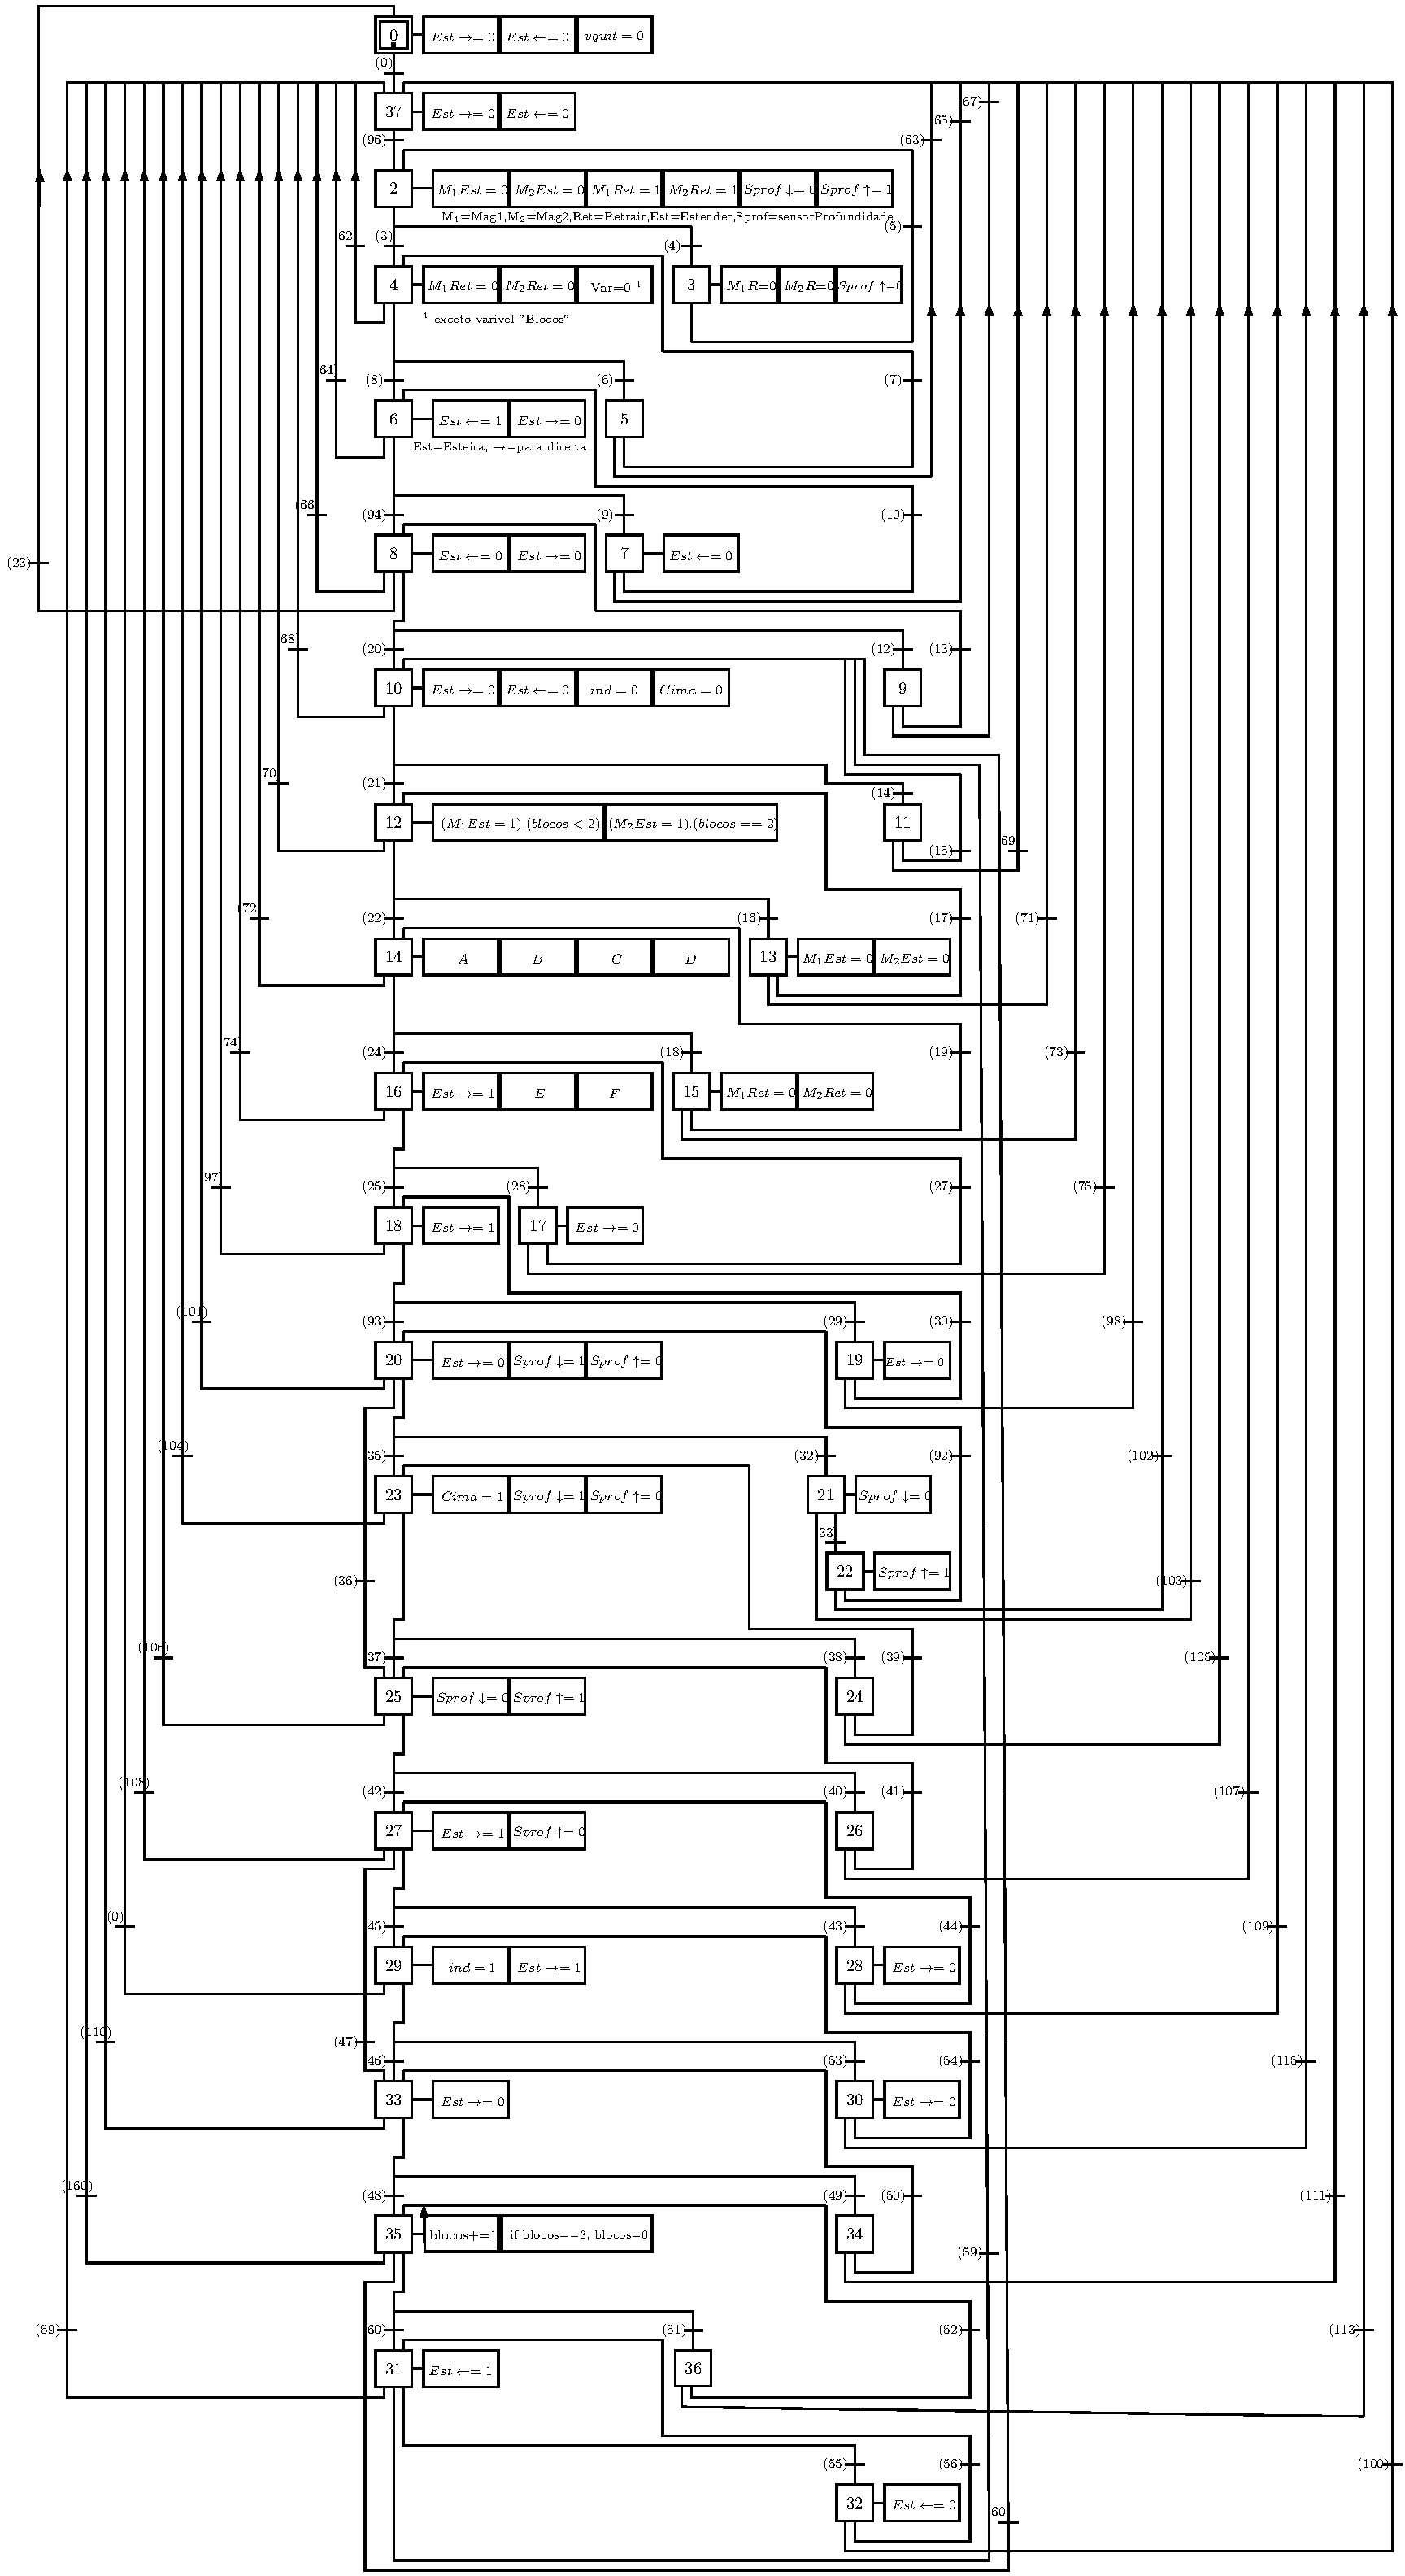
\includepdf[pages=-,width=320mm,offset=270 -425]{grafcet.pdf}
\eject \pdfpagewidth=210mm \pdfpageheight=297mm
\mysection{Ladder}
Para transformar da Rede de Petri mostrada na figura \ref{rededepetri} para o programa ladder, foi utilizado o algoritmo mostrado pelo o professor em aula. Devido ao uso dos stops e starts no problema, o programa foi modificado ligeiramente para não haver a necessidade de duplicar todos os estados e resultar numa rede de petri tão grande quanto a mostrada, com inúmeros lugares e muitas transições que fazem basicamente a mesma coisa (tirar fichas dos lugares onde estavam e colocando no lugar $P_{37}$, como mostrado na Network 63. \\

\mysection{Conclusão}
Como conclusão, pudemos perceber facilidade de modelar o sistema de controle de uma planta mecatrônica a partir de uma rede de petri e a eficiência da transformação da rede de petri para a linguagem ladder, que é utilizada na programação da maioria dos CLP's.





\appendix
  \mysection{Programa em Ladder}
  A seguir podemos ver todo o programa em Ladder construído para o funcionamento do controle a eventos discretos projetado.
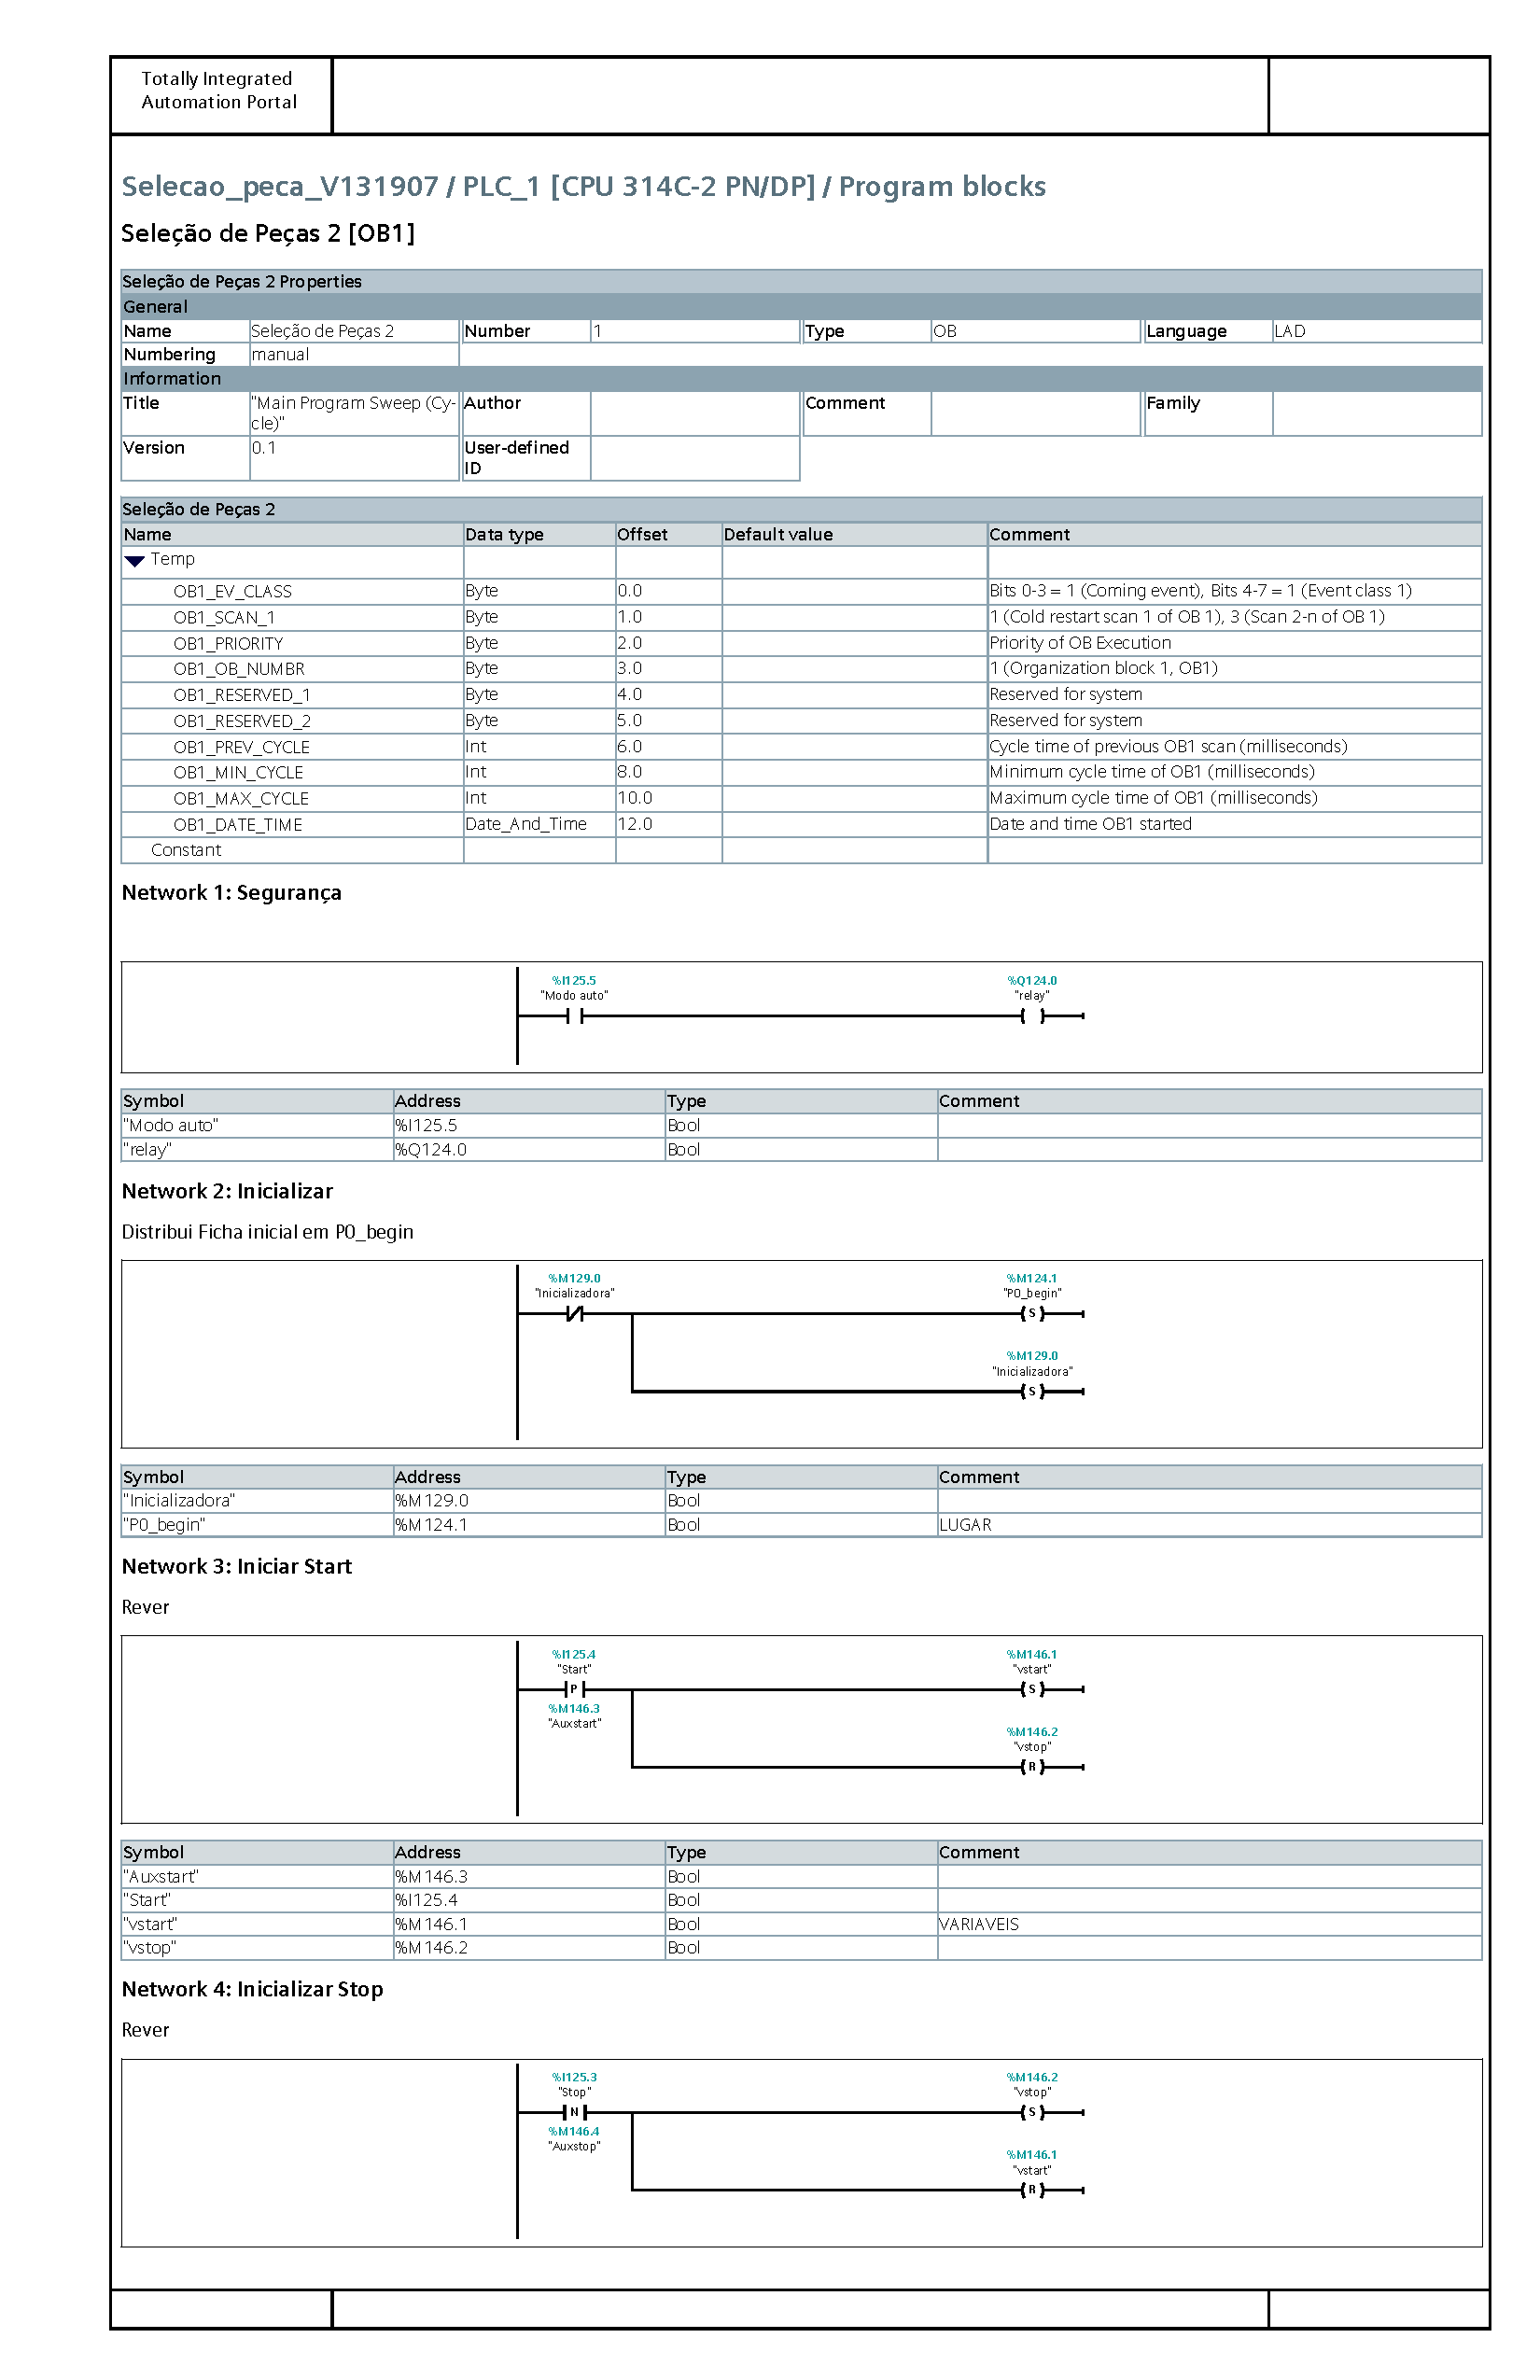
\includepdf[pages=-]{ladder.pdf}


\bibliographystyle{plain}
\bibliography{bibliografia}
\end{document}